% Copyright (C) Royal Astronomical Society 2015
% Authors:
% Keith T. Smith (Royal Astronomical Society)

%%%%%%%%%%%%%%%%%%%%%%%%%%%%%%%%%%%%%%%%%%%%%%%%%%
% Basic setup. Most papers should leave these options alone.
\documentclass[fleqn,usenatbib]{mnras}

% MNRAS is set in Times font. If you don't have this installed (most LaTeX
% installations will be fine) or prefer the old Computer Modern fonts, comment
% out the following line
\usepackage{newtxtext,newtxmath}
% Depending on your LaTeX fonts installation, you might get better results with one of these:
%\usepackage{mathptmx}
%\usepackage{txfonts}

% Use vector fonts, so it zooms properly in on-screen viewing software
% Don't change these lines unless you know what you are doing
\usepackage[T1]{fontenc}

% Allow "Thomas van Noord" and "Simon de Laguarde" and alike to be sorted by "N" and "L" etc. in the bibliography.
% Write the name in the bibliography as "\VAN{Noord}{Van}{van} Noord, Thomas"
\DeclareRobustCommand{\VAN}[3]{#2}
\let\VANthebibliography\thebibliography
\def\thebibliography{\DeclareRobustCommand{\VAN}[3]{##3}\VANthebibliography}


%%%%% AUTHORS - PLACE YOUR OWN PACKAGES HERE %%%%%

% Only include extra packages if you really need them. Avoid using amssymb if newtxmath is enabled, as these packages can cause conflicts. newtxmatch covers the same math symbols while producing a consistent Times New Roman font. Common packages are:
\usepackage{graphicx}	% Including figure files
\usepackage{amsmath}	% Advanced maths commands

%%%%%%%%%%%%%%%%%%%%%%%%%%%%%%%%%%%%%%%%%%%%%%%%%%

%%%%% AUTHORS - PLACE YOUR OWN COMMANDS HERE %%%%%

% Please keep new commands to a minimum, and use \newcommand not \def to avoid
% overwriting existing commands. Example:
%\newcommand{\pcm}{\,cm$^{-2}$}	% per cm-squared
\newcommand{\akira}[1]{\textcolor{red}{[AT: #1]}}

%%%%%%%%%%%%%%%%%%%%%%%%%%%%%%%%%%%%%%%%%%%%%%%%%%

%%%%%%%%%%%%%%%%%%% TITLE PAGE %%%%%%%%%%%%%%%%%%%

% Title of the paper, and the short title which is used in the headers.
% Keep the title short and informative.
\title[Lensing Super Sample Covariance]{LSSC: Lensing Super Sample Covariance}

% The list of authors, and the short list which is used in the headers.
% If you need two or more lines of authors, add an extra line using \newauthor
\author[A. Tokiwa et al.]{
Akira Tokiwa,$^{1, 2, 3}$\thanks{E-mail: akira.tokiwa@ipmu.jp}
Adrian Bayer,$^{1}$
Masahiro Takada$^{1, 2,3}$
Jia Liu$^{1, 3}$
\\
% List of institutions
$^{1}$Kavli Institute for the Physics and Mathematics of the Universe (WPI), 5-1-5 Kashiwanoha, Kashiwa-shi, Chiba, 277-8583, Japan\\
$^{2}$Department of Physics, The University of Tokyo, 7-3-1 Hongo, Bunkyo-ku, Tokyo 113-0033 Japan\\
$^{3}$Center for Data-Driven Discovery, Kavli IPMU (WPI), UTIAS, The University of Tokyo, Kashiwa, Chiba 277-8583, Japan
}

% These dates will be filled out by the publisher
\date{Accepted XXX. Received YYY; in original form ZZZ}

% Enter the current year, for the copyright statements etc.
\pubyear{2024}

% Don't change these lines
\begin{document}
\label{firstpage}
\pagerange{\pageref{firstpage}--\pageref{lastpage}}
\maketitle

% Abstract of the paper
\begin{abstract}
we study the effect of super sample covariance (SSC) on the weak lensing statistics. 
We use a set of N-body simulations to quantify the SSC effect on the convergence power spectrum, peak counts, minimum counts, and the scattering transform. 
We find that the SSC effect is negligible for the convergence power spectrum and higher order statistics.
We discuss the implication of our results for the future weak lensing surveys such as Euclid and Rubin Observatory Legacy Survey of Space and Time (LSST).
\end{abstract}

% Select between one and six entries from the list of approved keywords.
% Don't make up new ones.
\begin{keywords}
keyword1 -- keyword2 -- keyword3
\end{keywords}

%%%%%%%%%%%%%%%%%%%%%%%%%%%%%%%%%%%%%%%%%%%%%%%%%%

%%%%%%%%%%%%%%%%% BODY OF PAPER %%%%%%%%%%%%%%%%%%

\section{Introduction}

\section{Covariance}
\textbf{almost copy from the paper of \cite{PhysRevD.108.043521}}

The covariance matrix between an observable $\mathcal{O}_\alpha$ and another observable $\mathcal{O}_\beta$ is given by 
\begin{equation}
    C_{\alpha\beta} = \left(\left<\mathcal{O}_\alpha - \left<\mathcal{O}_\alpha\right>\right>\right)\left(\left<\mathcal{O}_\beta - \left<\mathcal{O}_\beta\right>\right>\right)
\end{equation}
$\left<\right>$ denotes the mean over the realizations. $C_{\alpha\beta}$ can be estimated by using an ensemble of simulations of different realizations of the initial conditions.

We quantify the SSC effect by comparing the following two sets of simulations:
\begin{itemize}
    \item lightcone of sub-boxes that extract from a much larger simulation box, captures super-sample mode $\theta > \theta_{max}$.
    \item lightcone of small-boxes that consists of tiled small boxes, independently simulated with periodic boundary conditions and only have mode $\theta \leq \theta_{max}$.
\end{itemize}

Because the Super sample modes are only present in the former and not in the latter, the SSC is given by 
\begin{equation}
    C_{SSC} = C_{sub} - C_{small}
\end{equation}
where $C_{sub}$ is the covariance computed using sub-boxes and $C_{small}$ is that using small boxes.

\section{Methods}
\label{sec:method}
We started by generating N-body simulations of $\boldsymbol{BIGBOX}$ and $\boldsymbol{TILED}$ and used them to generate full sky convergence maps. 
To measure the statistics in different scale, we smoothed the convergence maps with Gaussian filters of various scales.

\subsection{N-body Simulations}
The dark-matter only N-body simulations were done using the FASTPM. \akira{description of how good the FASTPM is}

Assuming a flat $\Lambda CDM$ cosmology with the following parameters: 
$\Omega_0 = 0.3089$, $\Omega_\Lambda = 0.6911$, $h = 0.6774$, $D = 0.12745536$ and $f = 0.99875922$. 
The $\boldsymbol{BIGBOX}$ has a side length of $L = 5000 Mpc/h$ and contains $8192^3$ particles.
The $\boldsymbol{TILED}$ consists of $8^3$ small boxes with a side length of $L = 625 Mpc/h$ and contains $1024^3$ particles.

\subsection{Generating Convergence Map}
Sitting at the corner of the simulation box, we can only generated a light cone covering one octant of the sky.
To generate a full sky map, we rotated the light cone to cover the full sky.

Snapshots are outputted from scale factor $a = 0.3$ to $a = 1.0$ with a spacing of $\Delta a = 0.01$.
That is, we have 71 snapshots from redshift $z = 0.0$ to $z = 2.3$.




\subsection{Ray Traced Weak Lensing Map}
\textbf{almost copy from the paper of \cite{10.1093/mnras/stab395}}

To build a light cone, we stacked the snapshots along the line-of-sight in an interval of $500 Mpc/h$, which is the size of the small boxes. 
The comoving distance is from $z=0$ to $z\sim1.65$.
We summarize the light cone configuration in table \ref{tab:config}.
Here, the redshift is simply computed by using the comoving distance of the snapshot center with \texttt{Python} package \texttt{astropy}.
The opening angle of the light cone is $5\times5\ \mathrm{deg}^2$. 
\begin{table}
    \centering
    \caption{Summary of the light cone. Columns (1) snapshot number; (2) comoving distance and (3)redshift at the snap shot center.}
    \label{tab:config}
    \begin{tabular}{ccc}
        \# Snapshot & $\chi [Mpc/h]$ & z \\ \hline\hline
        1 & 250 & 0.057 \\
        2 & 750 & 0.177 \\
        3 & 1250 & 0.305 \\
        4 & 1750 & 0.443 \\
        5 & 2250 & 0.593 \\
        6 & 2750 & 0.759 \\
        7 & 3250 & 0.942 \\
        8 & 3750 & 1.148 \\
        9 & 4250 & 1.382 \\
        10 & 4750 & 1.649 \\ \hline
    \end{tabular}
\end{table}

\begin{figure*}
    \centering
    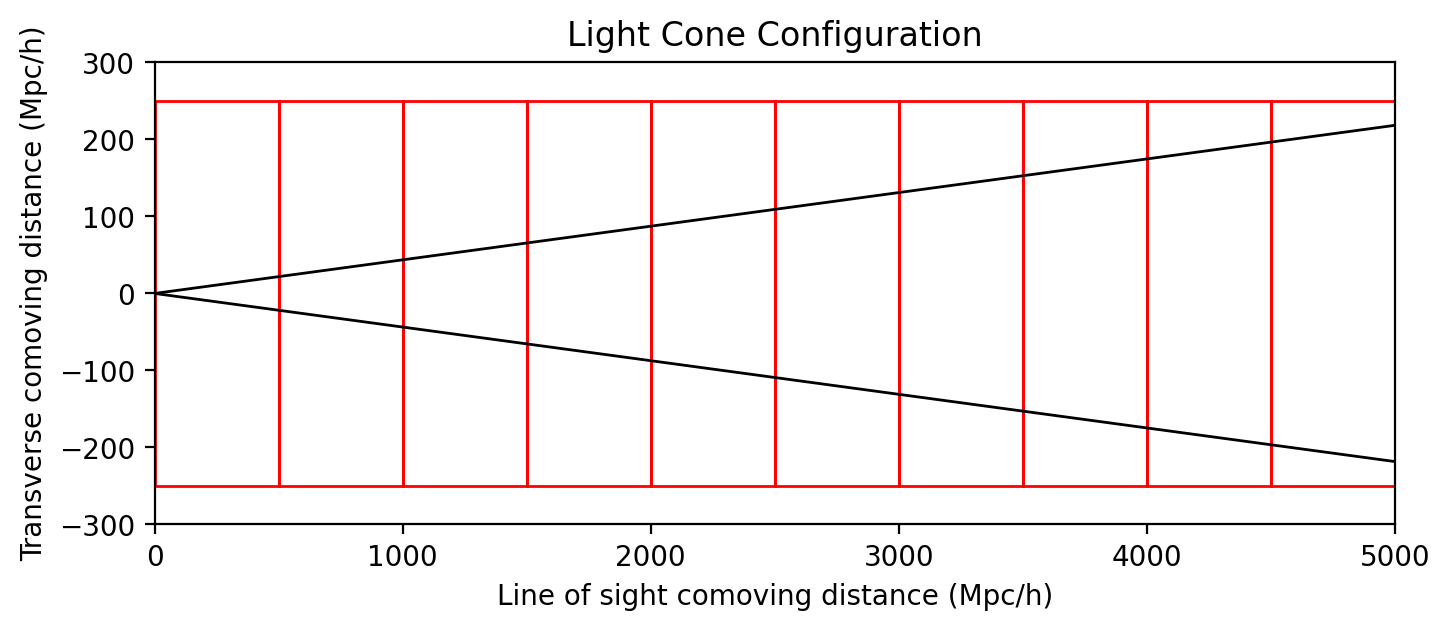
\includegraphics[width=0.95\hsize]{img/config.png}
    \caption{The construction of the light cone. Each red box corresponds to one snapshot. 
    The black lines correspond to the opening angle of 5 deg.}
    \label{fig:config}
\end{figure*}

To model the propagation of light rays, we employ a multiple lens plane approximation, 
where the smooth matter distribution is approximated as discrete density planes of thickness $\Delta \chi$.
Light rays originating from the observer at z = 0 are deflected only at the planes and travel in straight lines between the planes.
At the angular position  $\beta^k$  at the k-th plane, the deflection angle $\alpha$ is the gradient of the 2D lensing potential $\psi$.

\begin{equation}
    \alpha^k(\beta^k) = \nabla_{\beta^k} \psi^k(\beta^k)
\end{equation}

The lensing potential can be computed from the Poisson equation:

\begin{equation}
    \nabla^2_{\beta^k} \psi^k(\beta^k) = 2 \sigma^k(\beta^k),
\end{equation}

where the dimensionless surface density $\sigma^k$ is the projected matter distribution of the k-th lens plane:

\begin{equation}
    \sigma^k(\beta^k) = \frac{3 H^2_0 \Omega_m}{2 c^2} \frac{\chi^k}{a^k} \int_{\chi^k + \Delta \chi/2}^{\chi^k - \Delta \chi/2} \delta(\beta^k, \chi) \, d\chi,
\end{equation}

where c is the speed of light, a is the scale factor, and $\delta = \left(\rho - \bar{\rho} \right) /\bar{\rho}$ is the three-dimensional matter overdensity. 
The lensed position $\beta^k$ is the sum of previous deflection angles:

\begin{equation}
    \boldsymbol{\beta}^k(\boldsymbol{\theta})=\boldsymbol{\theta}-\sum_{i=1}^{k-1} \frac{\chi^k-\chi^i}{\chi^k} \boldsymbol{\alpha}^i\left(\boldsymbol{\beta}^i\right),(k=2,3, \ldots)
\end{equation}

where we impose $\boldsymbol{\beta}^0=\boldsymbol{\beta}^1=\boldsymbol{\theta}$.
By differentiating $\boldsymbol{\beta}^k$ with respect to $\boldsymbol{\theta}$, 
we obtain the Jacobian matrix $\mathcal{A}$:

\begin{equation}
    \mathcal{A}(\boldsymbol{\theta}, \chi)\equiv \frac{\partial \boldsymbol{\beta}}{\partial \boldsymbol{\theta}}(\boldsymbol{\theta}, \chi)=
    \left(\begin{array}{cc}
        1 - \kappa - \gamma_1 & -\gamma_2 + \omega \\
        -\gamma_2 - \omega & 1 - \kappa + \gamma_1
    \end{array}\right)
\end{equation}
where $\kappa$ is the convergence, $\gamma_1$ and $\gamma_2$ are the two components of the shear, 
and $\omega$ is the rotation.

We apply a fast Fourier transform (FFT) to equation (2) to obtain the derivatives of the lensing potential $\psi$ with respect to the angular position $\beta^k$.
We evaluate the deflection and the Jacobian matrix at the angular position $\beta^k$ and generate $\kappa$, $\gamma_1$, $\gamma_2$, and $\omega$ maps at the k-th lens plane.
Note that k-th lens plane contains the matter distribution from the range $\left( \chi^k - \Delta \chi/2, \chi^k + \Delta \chi/2 \right)$.
but observables are defined at $\chi^k$. Thus, the k-th source plane is placed at $\chi^k + \Delta \chi/2$.

\section{Statistics}
\begin{itemize}
    \item Convergence Power Spectrum: 
    Under flat sky approximation, the Fourier transform of the convergence map is defined by 
    \begin{equation}
        \kappa(\boldsymbol{\theta})=\int \frac{\mathrm{d}^2 \ell}{(2 \pi)^2} \mathrm{e}^{i \ell \cdot \theta} \tilde{\kappa}(\boldsymbol{\ell})
    \end{equation}
    The power spectrum of the convergence map is defined by
    \begin{equation}
        \left\langle\tilde{\kappa}\left(\boldsymbol{\ell}_1\right) \tilde{\kappa}\left(\boldsymbol{\ell}_2\right)\right\rangle=(2 \pi)^2 \delta_{\mathrm{D}}^{(2)}\left(\boldsymbol{\ell}_1-\boldsymbol{\ell}_2\right) P_{\kappa \kappa}\left(\ell_1\right)
    \end{equation}
    By using Limber approximation, the convergence power spectrum is described as follows:
    \begin{equation}
        P_{\kappa \kappa}(\ell)=\int_0^{\chi_s} \mathrm{~d} \chi \frac{W_\kappa(\chi)^2}{r(\chi)^2} P_\delta\left(k=\frac{\ell}{r(\chi)}, z(\chi)\right)
    \end{equation}
    where the lensing weight function is defined by
    
    \item PDF
    \item Peak
    \item minimum
    \item scattering transform
    \item Mass function
\end{itemize}

\subsection{Maths}

\section{Conclusions}



\section*{Acknowledgements}

The Acknowledgements section is not numbered. Here you can thank helpful
colleagues, acknowledge funding agencies, telescopes and facilities used etc.
Try to keep it short.

%%%%%%%%%%%%%%%%%%%%%%%%%%%%%%%%%%%%%%%%%%%%%%%%%%
\section*{Data Availability}

 
The inclusion of a Data Availability Statement is a requirement for articles published in MNRAS. Data Availability Statements provide a standardised format for readers to understand the availability of data underlying the research results described in the article. The statement may refer to original data generated in the course of the study or to third-party data analysed in the article. The statement should describe and provide means of access, where possible, by linking to the data or providing the required accession numbers for the relevant databases or DOIs.

\section{Citation}
\cite{Sato_2009}, \cite{2015MNRAS.453.3043S}


%%%%%%%%%%%%%%%%%%%% REFERENCES %%%%%%%%%%%%%%%%%%

\bibliographystyle{mnras}
\bibliography{main} 

%%%%%%%%%%%%%%%%%%%%%%%%%%%%%%%%%%%%%%%%%%%%%%%%%%

%%%%%%%%%%%%%%%%% APPENDICES %%%%%%%%%%%%%%%%%%%%%

\appendix

\section{Some extra material}

If you want to present additional material which would interrupt the flow of the main paper,
it can be placed in an Appendix which appears after the list of references.

%%%%%%%%%%%%%%%%%%%%%%%%%%%%%%%%%%%%%%%%%%%%%%%%%%


% Don't change these lines
\bsp	% typesetting comment
\label{lastpage}
\end{document}

% End of mnras_template.tex
